\chapter{先行事例}
\thispagestyle{fancy}

\section{先行事例}
プロジェクションマッピングを用いて,高い演出効果を生み出す先行事例としては,まず,建物への投影だ.
図\ref{disney}に,東京ディズニーランドで2014年5月から2017年11月まで行われた「Once upon a time」を示す.
シンデレラ城にマッピングをし,驚きと感動を届けた.
現在もシンデレラ城で新たなプロジェクションマッピングが行われている\cite{once}.
また,図\ref{rio}の2016年8月に開幕した「リオオリンピック」開閉会式でもプロジェクションマッピングは行われた. 
2万ルーメンのプロジェクターをメインに333台のプロジェクターが使用された.
開会式では、プロジェクションマッピングを駆使した美しい映像演出が反響を呼び、
南米初開催となったオリンピックを強く印象づけた\cite{olympic}.

次にライブやコンサートなどのイベントである.安室奈美恵は,二段構えの垂直のセット,
6面の縦長のビジョンを用い,ダンサー3人とプロジェクションマッピングが重なるような演出を行った\cite{amuro}.
また,Perfumeがフランス・カンヌで6月に開催された世界最大の広告祭
「カンヌライオンズ 国際クリエイティビティ・フェスティバル」でのパフォーマンスで,
プロジェクションマッピングを行った.3人がまとう真っ白な衣装がスクリーンとなり,
次々と色鮮やかなグラフィックが映し出された\cite{kirameku}.
このようにステージの背景だけでなく,アーティスト自身に投影を行うような例もある.

他にも,プロジェクションマッピングは,エンターテインメント分野だけでなく,
図\ref{syujutsu}のような,手術をリアルタイムでナビゲーションする装置\cite{iryou}など,
医療分野でも応用されている.


\clearpage

\begin{figure}[t]
  \centering
  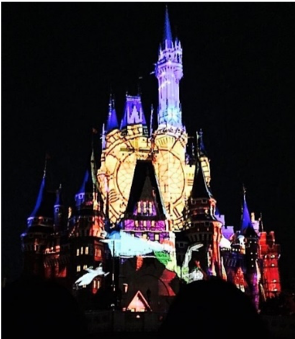
\includegraphics[width=9cm]{image/disney.png}
  \caption{東京ディズニーランド Once upon a time}
\label{disney}
\end{figure}

\begin{figure}[b]
    \centering
    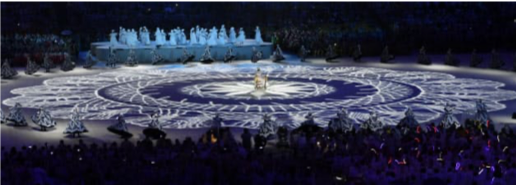
\includegraphics[width=9cm]{image/rio.png}
    \caption{リオオリンピック\cite{rioprojection}}
  \label{rio}
\end{figure}

\clearpage

\begin{figure}[t]
    \centering
    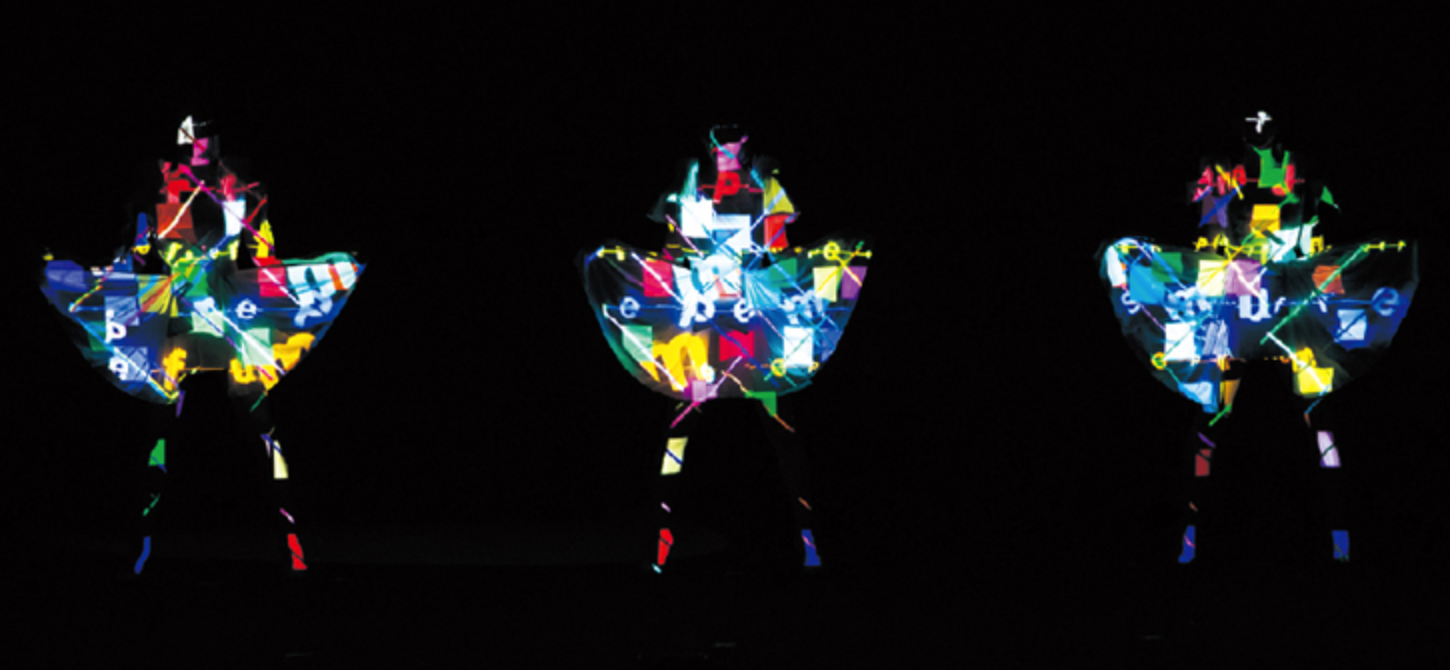
\includegraphics[width=9cm]{image/perfume1.png}
    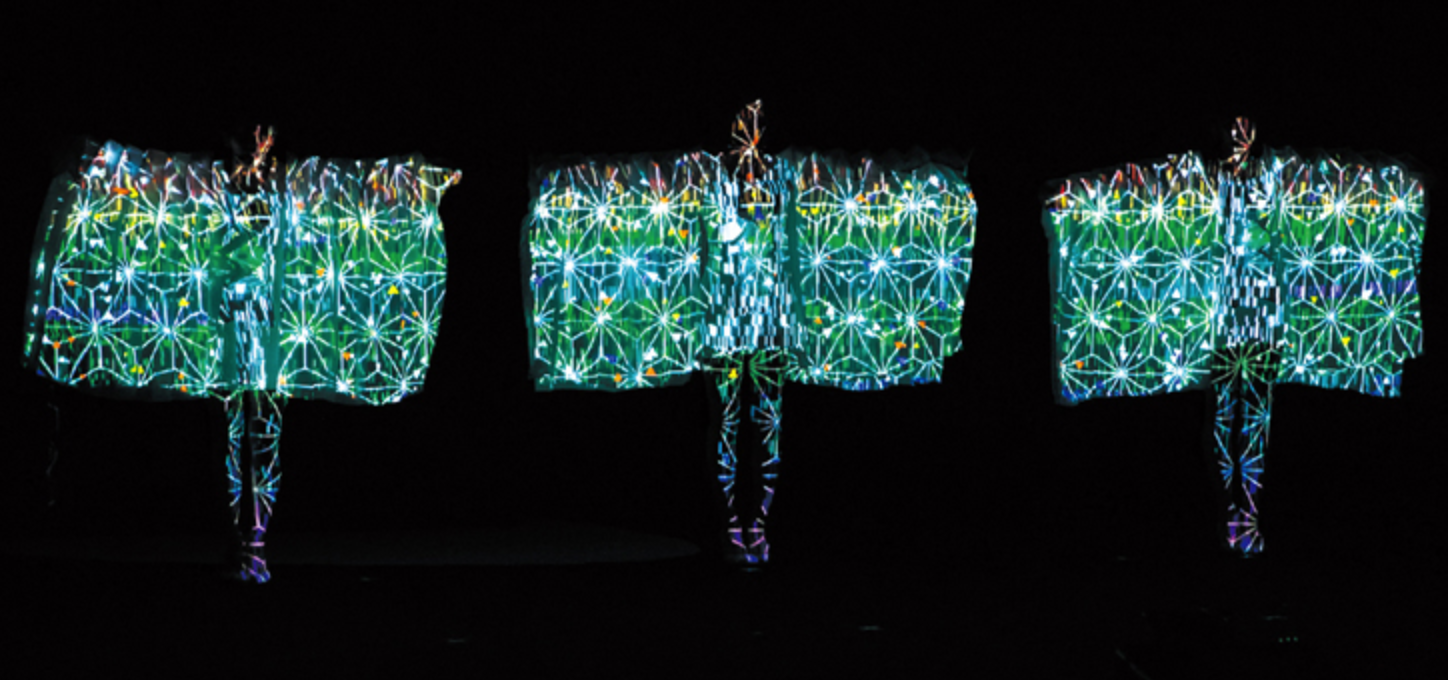
\includegraphics[width=9cm]{image/perfume2.png}
    \caption{Perfume カンヌライオンズ 
    \protect\linebreak 国際クリエイティビティ・フェスティバル\cite{kirameku}}
  \label{perfume}
\end{figure}



\begin{figure}[b]
  \centering
  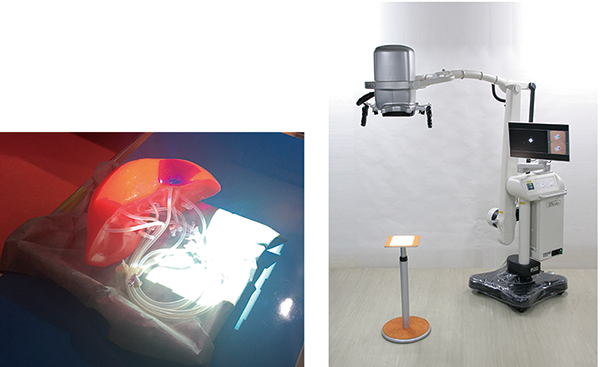
\includegraphics[width=9cm]{image/syujutsu.png}
  \caption{肝臓のICG発光をもとに切離線を決め,
  \protect\linebreak 修正しながら手術が可能\cite{iryou}}
\label{syujutsu}
\end{figure}

